\section{Problema 3: Heurística Constructiva Golosa}

\subsection{Descripción de la problemática}
En esta oportunidad se nos pide colaborar en la asignación de aulas con diversos recursos a un conjunto de materias (con un horario establecido e invariable) que necesitarían hacer uso de ellos durante el dictado de clase.\\
Como en este caso nos interesa distinguir las aulas de acuerdo a sus recursos, le asignaremos a cada una un color y uniremos con aristas aquellas materias que se han querido reservar para horarios cuya intersección no es vacía.\\
Dicho esto, nuestra tarea consiste en generar un algoritmo que implemente una heurística cuyo objetivo sea encontrar alguna forma de colorear los nodos (es decir, asignar a cada materia un aula ), minimizando en la medida de lo posible la cantidad de conflictos (entendidos estos como instancias que impiden que el coloreo generado sea válido, es decir, que verifique para toda arista que a sus nodos adyacentes se les haya asignado distinto color.) 


\subsection{Resolución propuesta y justificación}
Dos ideas de peso sugieron al proponernos resolver este problema:
\begin{itemize}
\item{Iterar sobre el grafo (a lo sumo C-1 veces) descartando de cada uno de los nodos uno de sus colores posibles, escogido mediante una función de peso que decidiera cuál de ellos podría generar más conflictos si se utilizara para colorear al nodo examinado.  }
\item{Realizar un barrido del grafo mediante BFS utilizando una función de peso similar a la mencionada que permitiera decidir para cada nodo cuál sería el color - potencialmente - de menor riesgo en una vecindad reducida y asignárselo. }
\end{itemize}

Un problema emergió al analizar la primera de las ideas: el hecho de que se realizaran varias iteraciones sobre el mismo grafo hacía que al comenzar cada una de ellas cada nodo tuviese más información del grafo completo que la que podía verificar en la anterior. Dicho de otra forma: en la primera iteración cada nodo tomaba la mejor decisión posible en función de su vecindad de primer nivel, pero en las siguientes ya dicha vecindad - ahora modificada de acuerdo a su propio entorno - le proveía al nodo más datos que los alcanzables hasta entonces. Es decir, no cumplía los requisitos para ser catalogado como ``algoritmo goloso''.\\
Es por esto que se decidió implementar la segunda opción, la cuál se explica a continuación:\\
Supóngase que se tiene el siguiente grafo, donde los números dentro de cada nodo indican su índice y los que se encuentran fuera enumeran sus colores posibles.\\

 \begin{figure}[H]
    \begin{center}
  	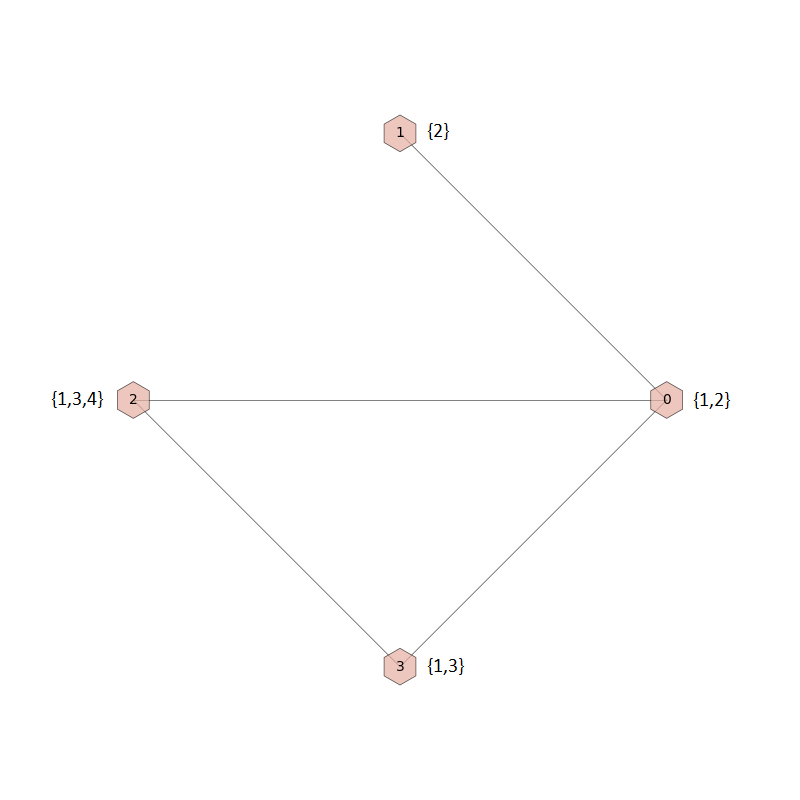
\includegraphics[width=13cm]{imagenes/Ej3/4Nodos0.png}
 	\caption{Grafo sin colorear}
 	\label{sinColor}
    \end{center}
  \end{figure}


Defínase Peso(N$_{c}$) como la función que determina la magnitud del perjuicio ocasionable al elegir colorear el nodo N de color c (con c $\epsilon$ \{colores de N\}), ${X}_{(c,p)}$ como el valor relativo X del color c para el nodo p. Entonces en un primer paso, los valores son los siguientes: 

\begin{itemize}
	\item \textbf{Nodo 0}
	\begin{itemize}
		\item Color 1:
		\begin{itemize}
			\item  $\frac{0}{1}_{(1,1)}$
			\item  $\frac{1}{3}_{(1,2)}$
			\item  $\frac{1}{2}_{(1,3)}$
		\end{itemize}

		\item Color 2:
		\begin{itemize}
			\item  $\frac{1}{1}_{(2,1)}$
			\item  $\frac{0}{3}_{(2,2)}$
			\item  $\frac{0}{2}_{(2,3)}$
		\end{itemize}
	\end{itemize}
\end{itemize}

Por lo tanto, \\
Peso(0$_{1}$) =  $\frac{ \frac{1}{2}_{(1,3)}}{\textbf{2}}$ + $\frac{\frac{1}{3}_{(1,2)}}{\textbf{3}}$ + $\frac{\frac{0}{1}_{(1,1)}}{\textbf{4}}$ $\simeq$ 0.36 \\
Peso(0$_{2}$) =  $\frac{\frac{1}{1}_{(2,1)}}{\textbf{2}}$ + $\frac{\frac{0}{3}_{(2,2)}}{\textbf{3}}$ + $\frac{\frac{0}{2}_{(2,3)}}{\textbf{4}}$ $\simeq$  0.5 \\
\newline
Como Peso(0$_{1}$) $\leq$  Peso(0$_{2}$), el color del que se pintará al nodo es del 1 (tal como se muestra en la \newline 
figura \ref{1color} )

 \begin{figure}[H]
    \begin{center}
  	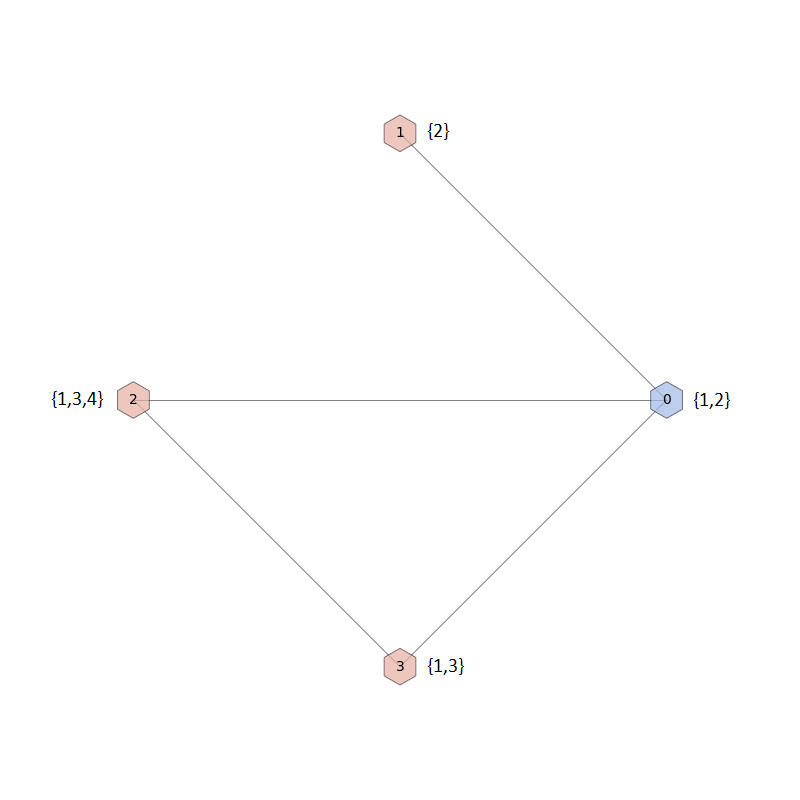
\includegraphics[width=13cm]{imagenes/Ej3/4Nodos1.png}
 	\caption{Al nodo 0 se le asigna el color 1}
 	\label{1color}
    \end{center}
  \end{figure}

Prosigamos con el nodo 1. Su valor es el siguiente:

\begin{itemize}
	\item \textbf{Nodo 1}
	\begin{itemize}
		\item Color 2:
		\begin{itemize}
			\item  $\frac{0}{2}_{(2,0)}$ 
		\end{itemize}
	\end{itemize}
\end{itemize}

Nótese que el valor $\frac{0}{2}_{(2,0)}$ no es $\frac{1}{2}_{(2,0)}$ porque el nodo 0 ya fue coloreado y de un color distinto al 2. Es por esto que al nodo 0 ``no le importa'' que su vecino, el nodo 1, se coloree del color 2 y por lo tanto el peso que retorna para dicho color es \textit{0}. Además, este es el único peso que tiene en cuenta el nodo 1, puesto que no tiene más nodos adyacentes ni otros colores disponibles. Por lo tanto, como se muestra en la figura \ref{2colores}, el nodo 1 se pinta del color 2.

 \begin{figure}[H]
    \begin{center}
  	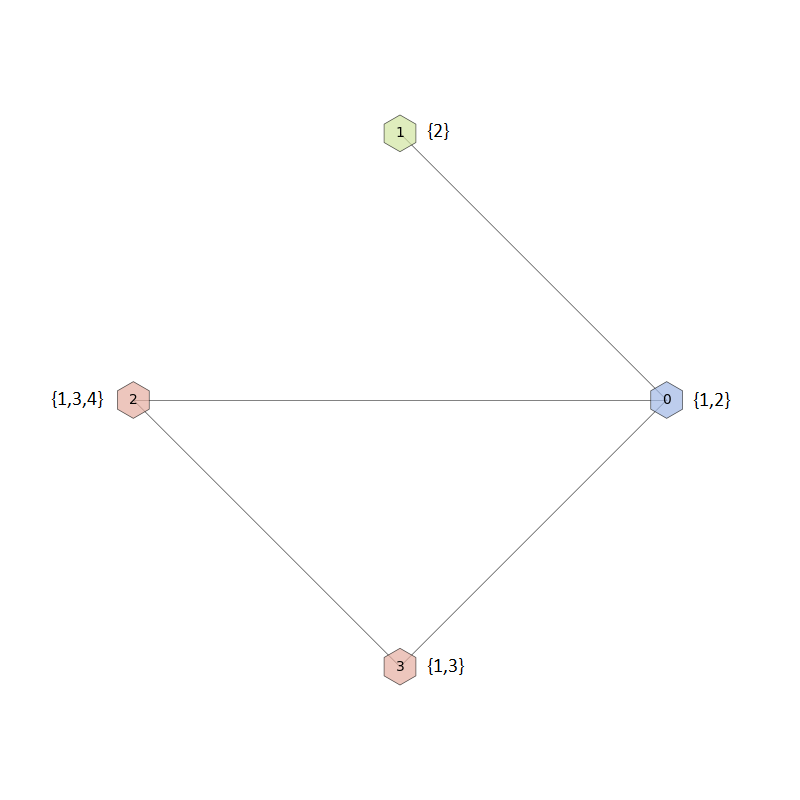
\includegraphics[width=13cm]{imagenes/Ej3/4Nodos2.png}
 	\caption{Al nodo 1 se le asigna el color 2}
 	\label{2colores}
    \end{center}
  \end{figure}

Continuemos el coloreo con el nodo 2: \\

\begin{itemize}
	\item \textbf{Nodo 2}
	\begin{itemize}
		\item Color 1:
		\begin{itemize}
			\item  $\frac{0}{2}_{(1,0)}$
			\item  $\frac{1}{2}_{(1,3)}$
		\end{itemize}

		\item Color 3:
		\begin{itemize}
			\item  $\frac{0}{2}_{(3,0)}$
			\item  $\frac{1}{2}_{(3,3)}$
		\end{itemize}

		\item Color 4:
		\begin{itemize}
			\item  $\frac{0}{2}_{(4,0)}$
			\item  $\frac{0}{2}_{(4,3)}$
		\end{itemize}
	\end{itemize}
\end{itemize}

Nuevamente, los colores posibles del nodo 0 no tienen injerencia a menos que el valor por el que se pregunte sea equivalente al color con el cual se pretende colorear un nodo adyacente.\\
Como en este caso  Peso(2$_{4}$) $\leq$  Peso(2$_{3}$)  $\leq$  Peso(2$_{1}$), se le asigna al nodo 2 el color 4 (ver \ref{3colores})

 \begin{figure}[H]
    \begin{center}
  	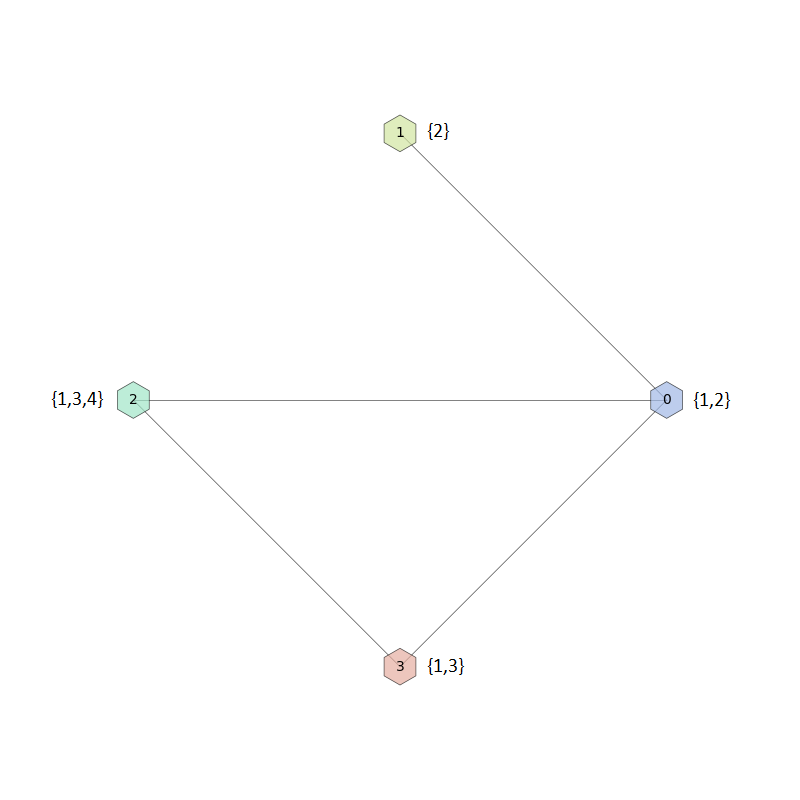
\includegraphics[width=13cm]{imagenes/Ej3/4Nodos3.png}
 	\caption{Al nodo 2 se le asigna el color 4}
 	\label{3colores}
    \end{center}
  \end{figure}

Por último, definamos el coloreo del nodo 3:\\

\begin{itemize}
	\item \textbf{Nodo 3}
	\begin{itemize}
		\item Color 1:
		\begin{itemize}
			\item  $\frac{1}{1}_{(1,0)}$
			\item  $\frac{0}{3}_{(1,2)}$
		\end{itemize}

		\item Color 3:
		\begin{itemize}
			\item  $\frac{0}{2}_{(3,0)}$
			\item  $\frac{0}{3}_{(3,2)}$
		\end{itemize}
	\end{itemize}
\end{itemize}

Obsérvese que $\frac{1}{1}_{(1,0)}$ es distinto del esperado $\frac{1}{2}_{(1,0)}$. Esto se debe a que ell valor escogido representa una medida de la importancia que se le da al nodo ya coloreado ``0''. Como queremos evitar la mayor cantidad de conflictos, ante casos de este estilo se define que el nodo coloreado retorne el valor absoluto ``1'' (recordemos que, cuanto más grande este valor, mayor es la restricción de pintar un nodo de dicho color).\\

De esta forma, queda coloreado todo el grafo como se muestra en la figura \ref{4colores}

 \begin{figure}[H]
    \begin{center}
  	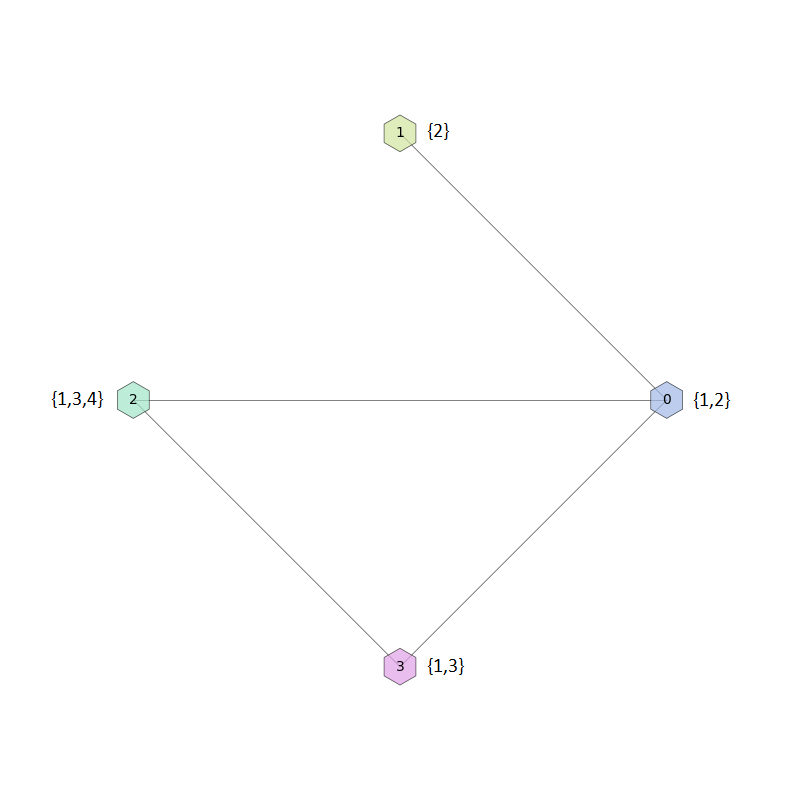
\includegraphics[width=13cm]{imagenes/Ej3/4Nodos4.png}
 	\caption{Al nodo 3 se le asigna el color 3}
 	\label{4colores}
    \end{center}
  \end{figure}


% \subsection{Código fuente}

% A continuación se incluyen las partes más relevantes del código generado\\

% La clase \emph{Lector.java} se encarga de tomar los datos del archivo de entrada y procesarlos para construir el grafo mediante el método \textit{MakeGraph()}:\\

% \begin{lstlisting}
% 	public Grafo MakeGraph() throws IOException 
% 	{
% 		Grafo grafo = new Grafo();
% 		int[] nodosAristasColores = Ej3Utils.ToIntegerArray(this.getArchivo().readLine().split(" "));
% 		grafo.cantidadDeNodos = nodosAristasColores[0];
% 		grafo.setCantidadDeAristas(nodosAristasColores[1]);
% 		grafo.setCantidadDeColores(nodosAristasColores[2]);
		
% 		try { grafo.setNodos(this.ObtenerListaDeNodos(grafo.cantidadDeNodos, grafo.getCantidadDeColores()));} 
% 		catch (IOException e) { System.out.println("Se produjo un error al generar los nodos del grafo.");}
% 		boolean[][] matrizDeAdyacencia = GenerarMatrizDeAdyacencia(grafo.getCantidadDeNodos(), grafo.getCantidadDeAristas(), false);
% 		grafo.setListaDeAdyacencia(Ej3Utils.matrizDeAdyacenciaToListDeAdyacencia(matrizDeAdyacencia, grafo.getNodos()));
		
% 		return grafo;
% 	}
		
% \end{lstlisting}


% La clase \emph{Grafo.java} contiene el método \textit{MakeRainbow()} que colorea el grafo con la heurística \newline propuesta: \\

% \begin{lstlisting}
% 	public void MakeRainbow() // O(n^2*c*log(n))
% 	{
% 		int nodosPintados = 0;
% 		LinkedList<Nodo> colaNodos = new LinkedList<Nodo>();

% 		while(nodosPintados < this.cantidadDeNodos)
% 		{
% 			colaNodos.add(PicANode(this)); //O(1)
			
% 			while (!colaNodos.isEmpty()) //O(n)
% 			{
% 				Nodo nodoActual = colaNodos.removeFirst(); //O(1)
				
% 				if (!nodoActual.isVisitado())
% 				{
% 					colaNodos.addAll(this.getVecinosDe(nodoActual)); //O(n)
% 					LinkedList<Integer> coloresRestantes = nodoActual.getColoresRestantes(); //O(1)
% 					PintarNodo(nodoActual, coloresRestantes, this); //O(c*n*log(n))
% 					nodosPintados ++;
% 					nodoActual.setVisitado(true); //O(1)
% 				}
% 			}
% 		}
% 	}
	
% 	private static Nodo PicANode(Grafo grafo) 
% 	{
% 		Nodo next = new Nodo();
% 		for(Nodo nodo : grafo.getNodos())
% 		{
% 			if (!nodo.isVisitado())
% 			{
% 				next = nodo;
% 				break;
% 			}
% 		}
% 		return next;
% 	}
	
% 	private static void PintarNodo(Nodo nodoActual, LinkedList<Integer> coloresRestantes, Grafo grafo) //O(c*n*log(n))
% 	{
% 		int colorAPintar = CalcularColorMenosPerjudicial(nodoActual, grafo); //O(c*n*log(n))
% 		nodoActual.setColor(colorAPintar); 
% 	}

% 	private static int CalcularColorMenosPerjudicial(Nodo nodoActual, Grafo grafo) //O(c*n*log(n))
% 	{
% 		Double pesoColor = 1.0;
% 		int colorAPintar = -1;
% 		for (int color : nodoActual.getColoresRestantes()) //O(c)
% 		{
% 			Double peso = CalcularPeso(color, grafo.getVecinosDe(nodoActual)); //O(nlog(n))
% 			if (peso <= pesoColor)
% 			{
% 				pesoColor = peso;
% 				colorAPintar = color;
% 			}	
% 		}	
% 		return colorAPintar;
% 	}


% 	private static Double CalcularPeso(int color, List<Nodo> vecinos) 
% 	{
% 		ArrayList<Double> pesos = new ArrayList<Double>();
% 		for (Nodo nodo : vecinos) //O(n)
% 		{
% 			if (nodo.LeImportaQueSuVecinoSePinteDelColor(color)) //O(1)
% 					pesos.add(nodo.PeligroDePintarUnVecinoDelColor(color));//O(1)(amortizado)
					
% 		}
% 		Collections.sort(pesos); //O(nlog(n))
% 		Double pesoTotal = 0.0;
% 		for (int k = 0; k < pesos.size(); k++) //O(n)
% 			pesoTotal += pesos.get(k)/(k+2); //O(1)
		
% 		return pesoTotal;
% 	}
		
% \end{lstlisting}


\subsection{PseudoCódigo y Análisis de la complejidad}

A continuación se presenta el pseudocódigo del coloreo implementado:

\begin{algorithmic} 
\WHILE{nodos pintados $\leq$ cantidad de nodos //O(n)} 
	\STATE {Elegir un nodo no visitado del grafo // O(n)}
	\STATE {Encolarlo //O(1)}
	\WHILE{hay elementos en la cola}  
		\STATE {Tomar el primer elemento de la cola //O(1)}
		\IF {no fue coloreado //O(1) } 
			\STATE{ Agregar a todos sus vecinos a la cola //O(n)}
			\STATE {Pintar nodo //O(n*c*log(n))}
		\ENDIF
	\ENDWHILE
\ENDWHILE
\end{algorithmic}


El ciclo principal (el externo) tiene razón de ser porque dentro del bucle anidado sólo se colorea una componente conexa por el grafo que recibimos puede ser no conexo, por lo tanto debemos iterar sobre las distintas componentes. Verificando que el algoritmo funcione hasta que la cantidad de nodos pintados sea efectivamente la cantidad de nodos total, y escogiendo cada vez un nodo de una componente no visitada podemos asegurarnos de que el coloreo se realiza sobre la totalidad del grafo.\\
El método \textit{PintarNodo()} tiene como cota superior O(n*c*log(n)). Como se puede ver en el código, dicha complejidad la alcanza al calcular el color menos perjudicial (método \textit{CalcularColorMenosPerjudicial(nodo V,grafo G)}). Mediante el mismo, se calcula el peso de cada color posible C de V mediante la verificación de la existencia de C entre el conjunto de los colores posibles de cada uno de sus nodos adyacentes a V. Gracias a que cada nodo lleva un array de booleanos que responde a dicha operación en O(1), la cota no es mayor.\\
Como la condición de que el nodo no haya sido visitado se valida exactamente n veces y cada vez se agregan a lo sumo n-1 elementos a la cola (con un costo O(1) cada uno), dicha parte del algoritmo cuesta O(n$^{2}$). Sin embargo un costo mayor se paga al ejecutar el método \textit{PintarNodo()}: n veces O(n*c*log(n)) . Esto hace que la complejidad final del algoritmo ascienda a O(n$^{2}$*c*log(n)).

\subsection{Experimentación}
Nos interesa analizar cómo se comporta nuestro algoritmo en función de ciertas características del grafo a ser coloreado: su cantidad de nodos, su cantidad de aristas y el número máximo de colores que puede llegar a tener como opción cada uno de sus nodos.\\
 Es por ello que nuestro primer experimento consistió en evaluar el tiempo necesario para el cómputo de distintos grafos en los cuales se incrementó paulatinamente la cantidad de nodos. Los resultados se pueden observar en la figura \ref{nodostiempo}

 \begin{figure}[H]
    \begin{center}
  	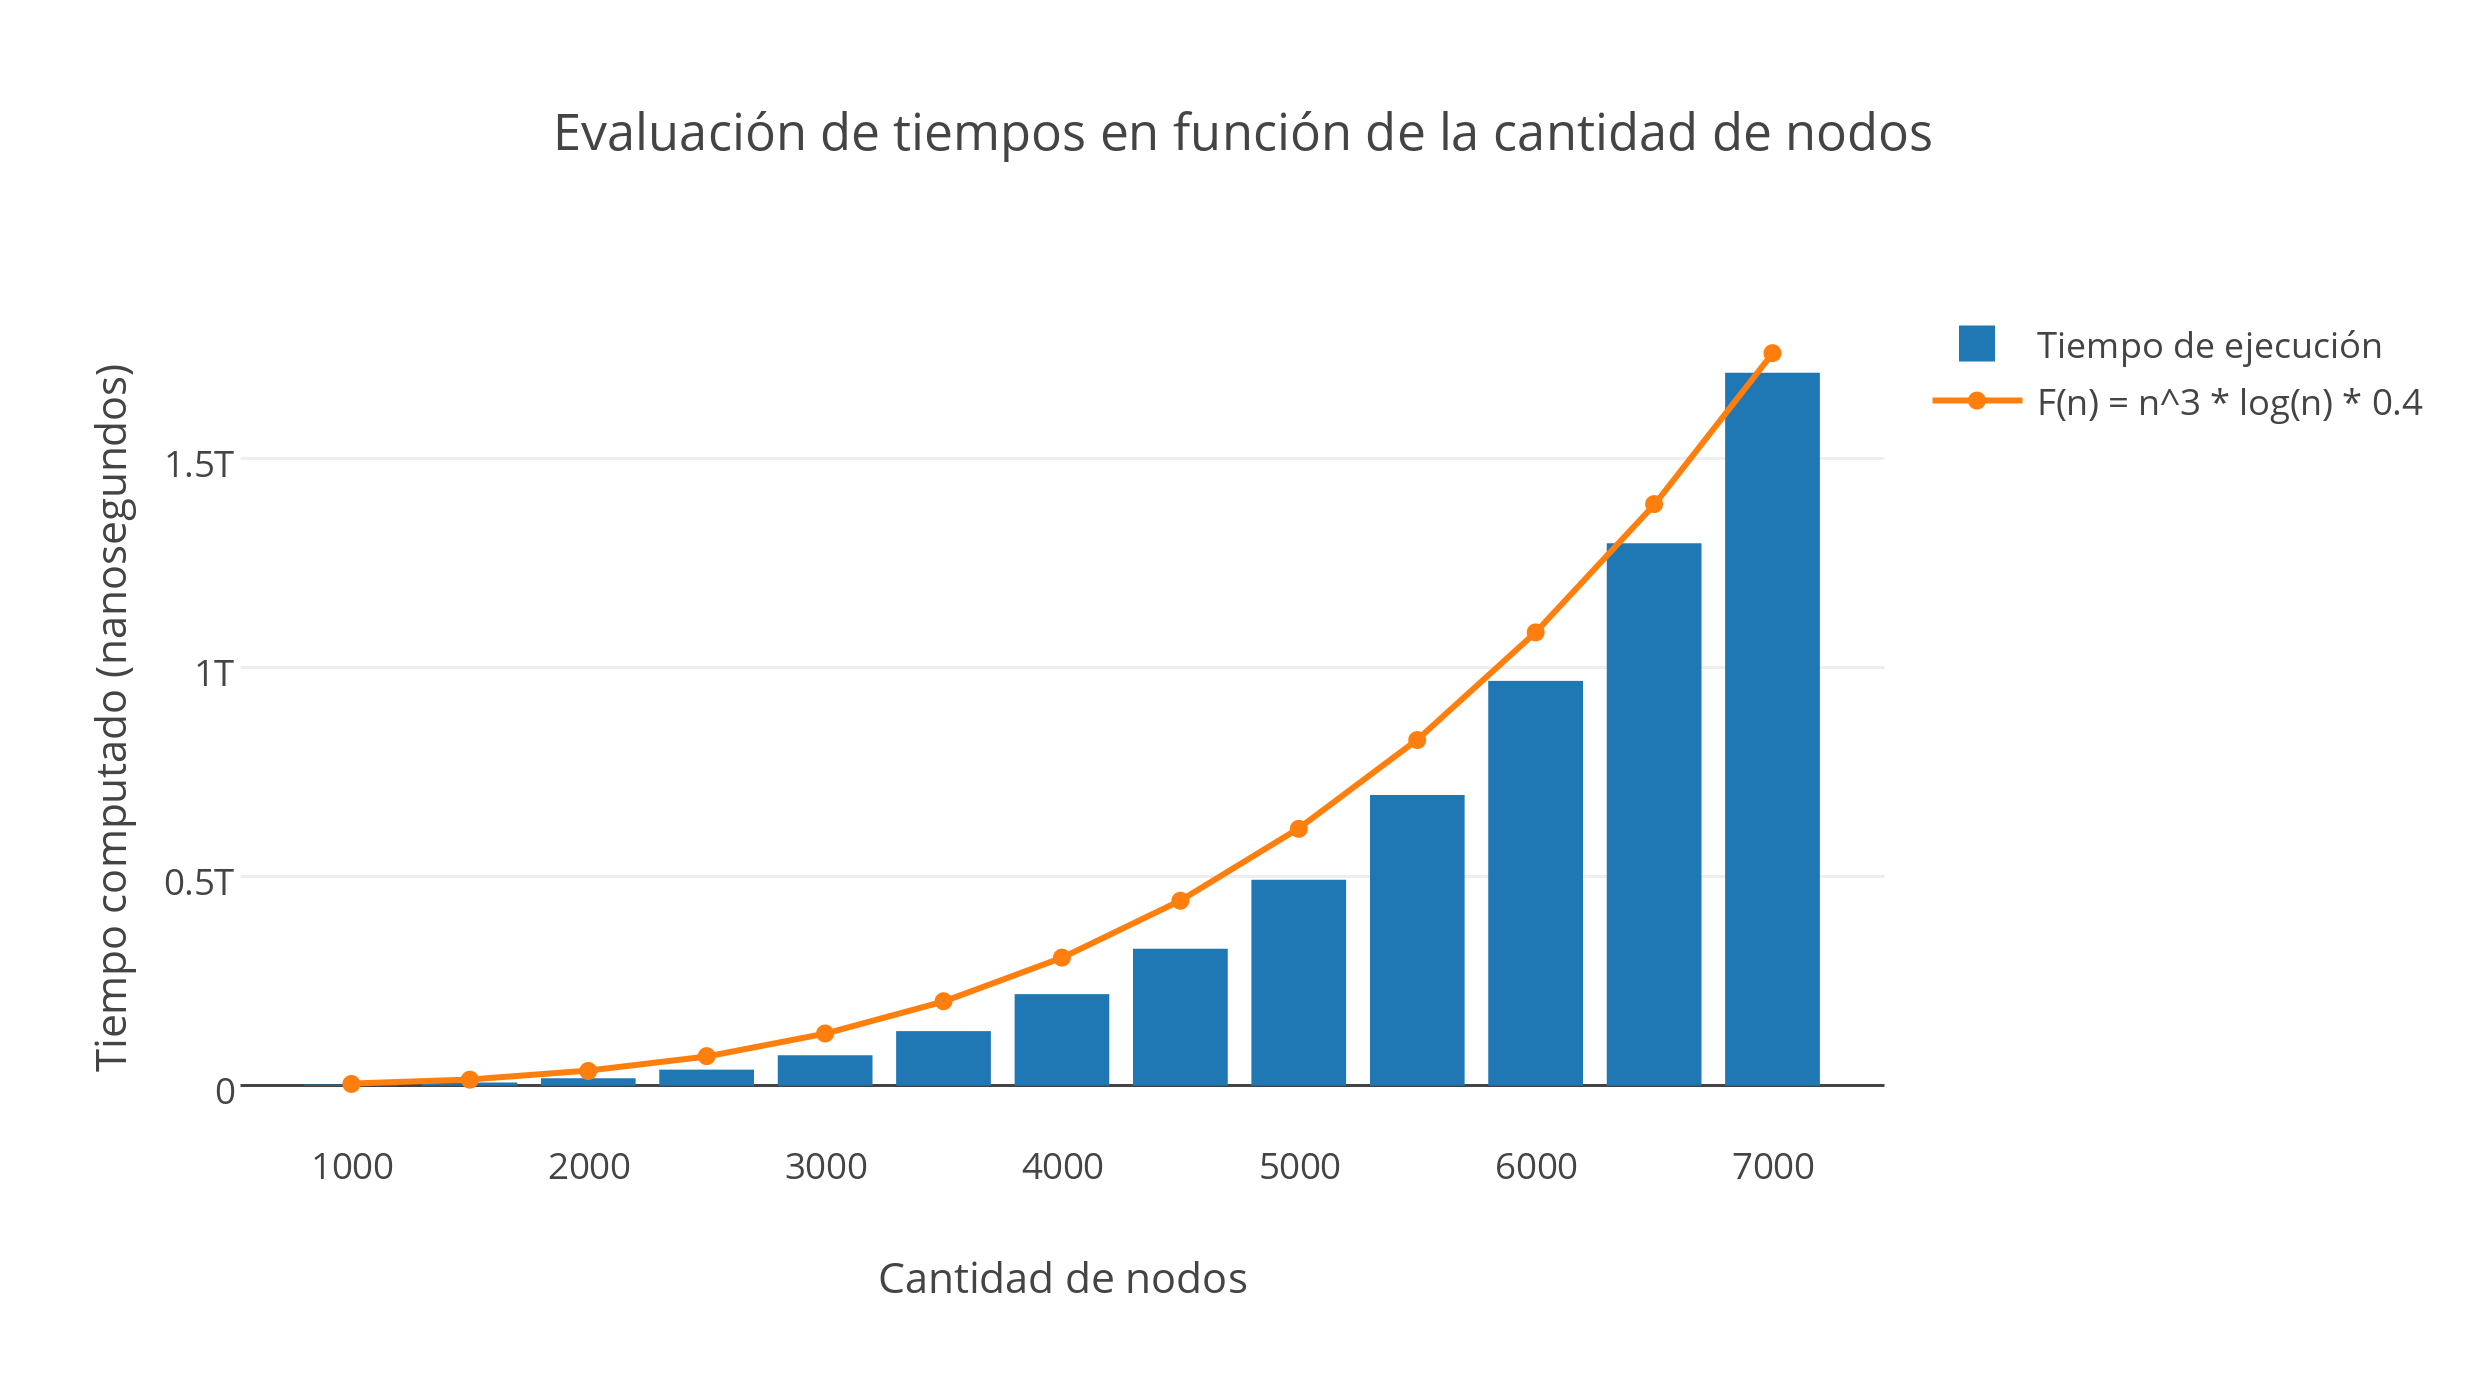
\includegraphics[width=18cm]{imagenes/Ej3/nodostiempo.png}
 	\caption{Tiempos de cómputo en función de la cantidad de nodos}
 	\label{nodostiempo}
    \end{center}
  \end{figure}

Como se puede observar, la función que permite acotar los resultados obtenidos se aproxima asintóticamente a los calculados previamente en forma teórica para estas instancias.\\
Por otro lado, generamos grafos que diferían entre sí únicamente en su cantidad de aristas. Al medir los tiempos obtuvimos los resultados que se exponen en la figura \ref{aristastiempo}

 \begin{figure}[H]
    \begin{center}
  	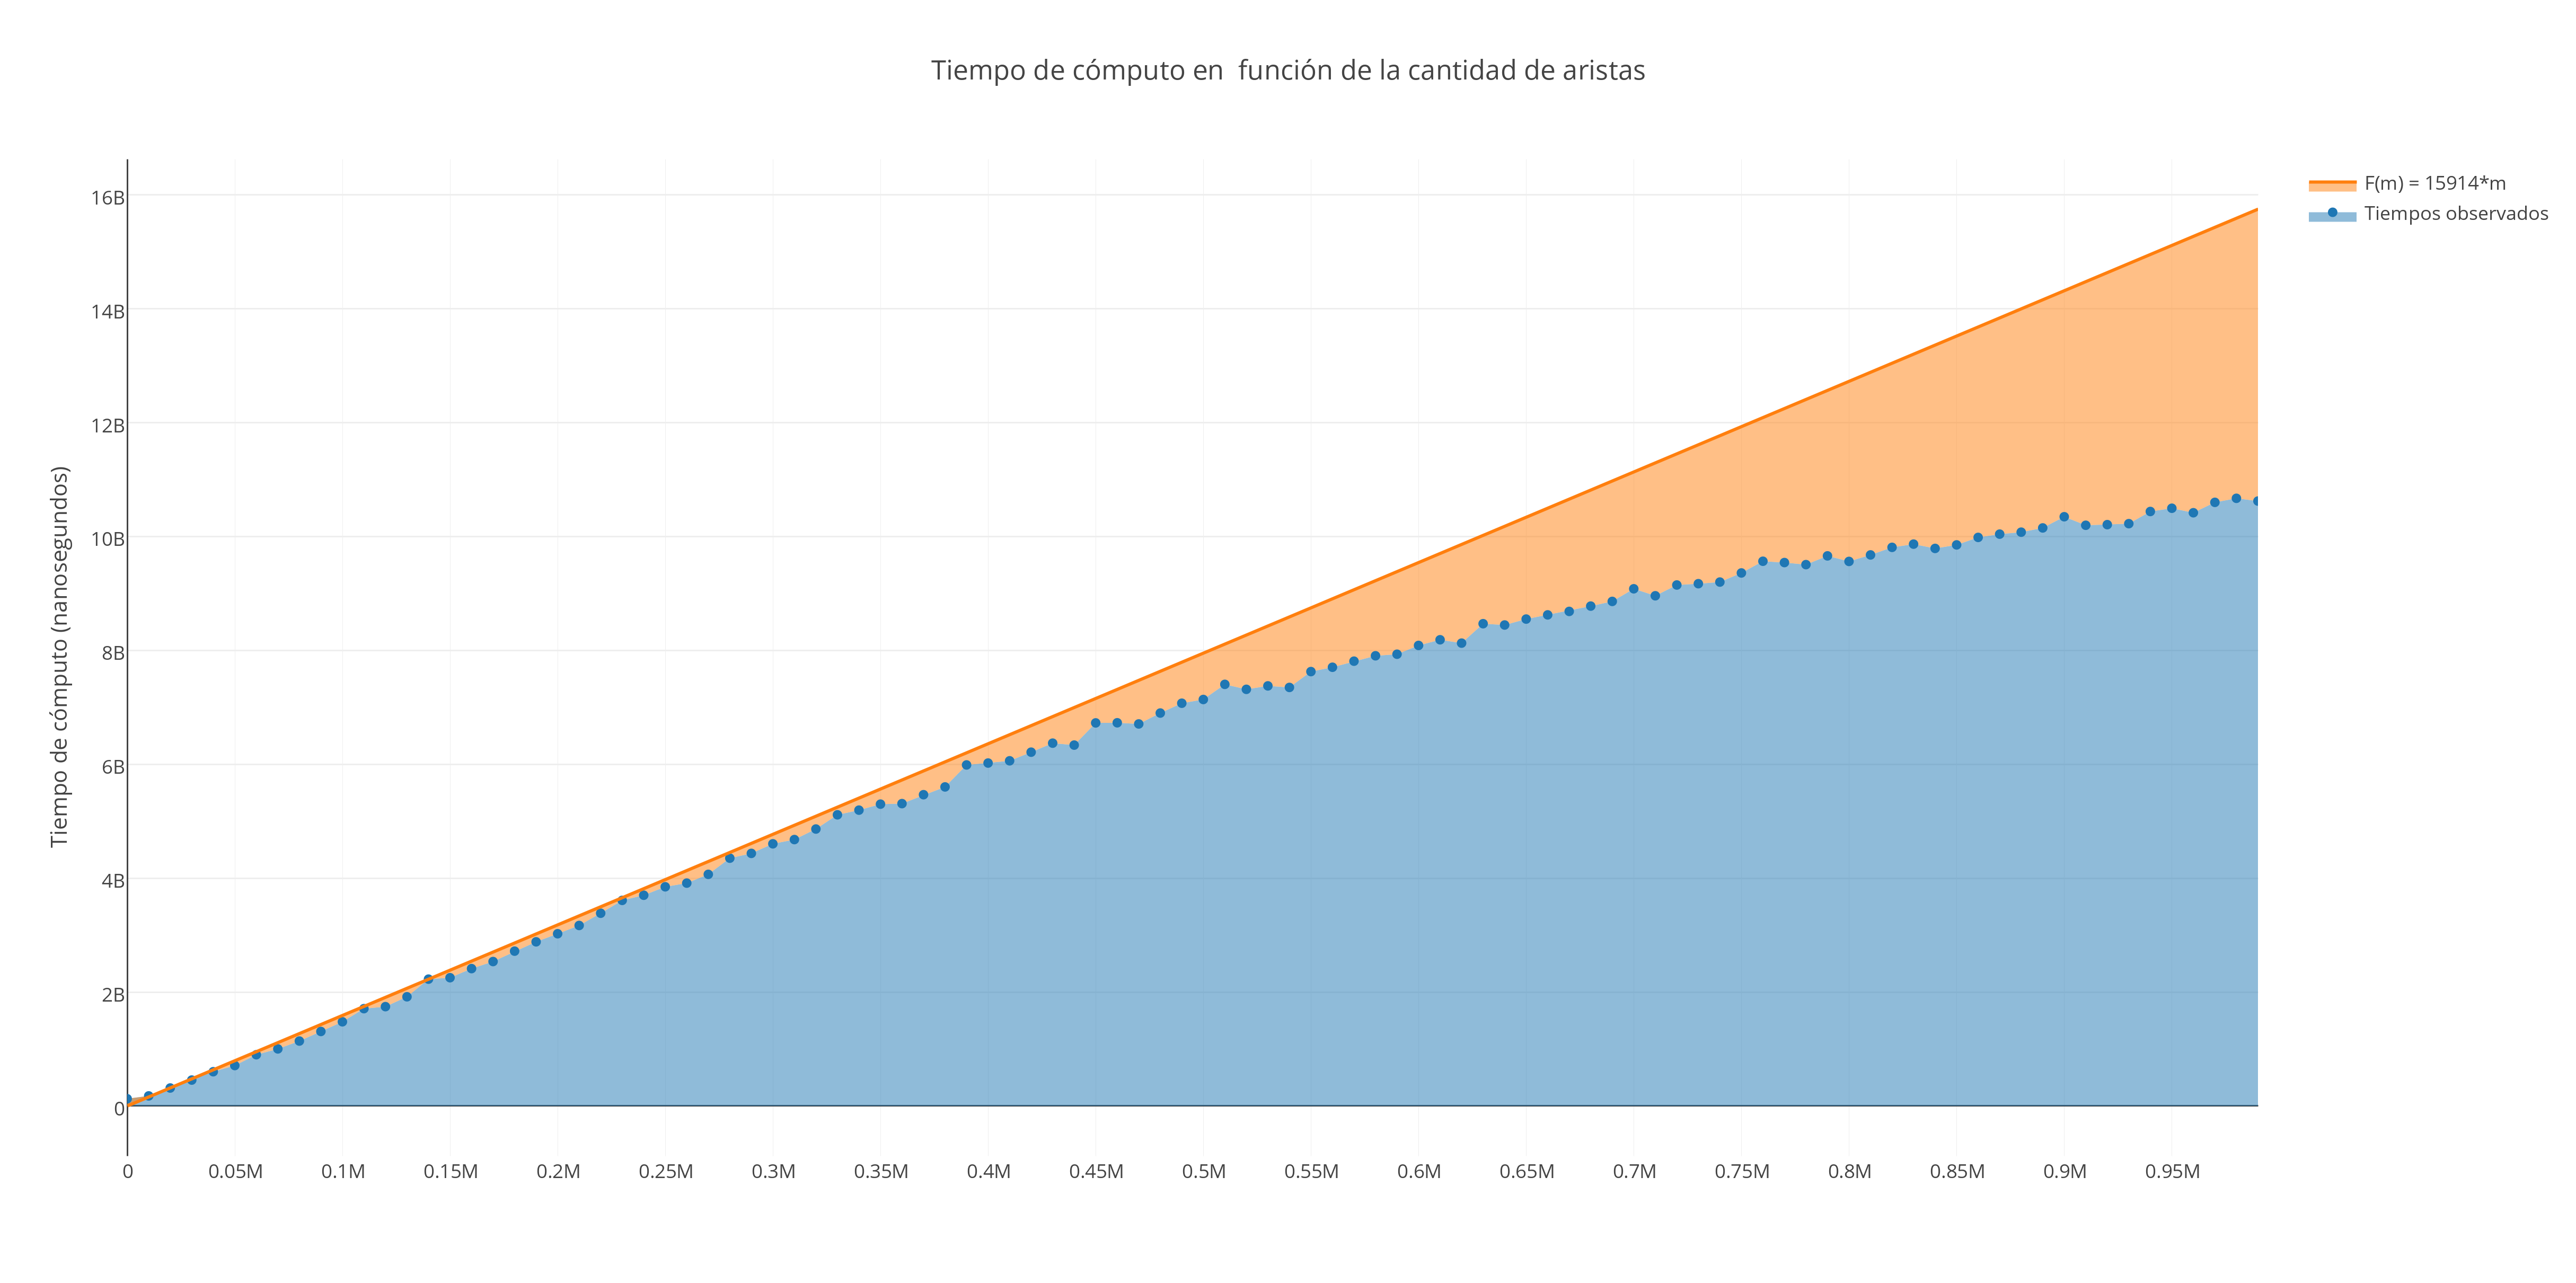
\includegraphics[width=18cm]{imagenes/Ej3/aristastiempo.png}
 	\caption{Tiempos de cómputo en función de la cantidad de aristas}
 	\label{aristastiempo}
    \end{center}
  \end{figure}

Así mismo, realizamos una serie de experimentos en los que modificamos para cada grafo la cantidad máxima de colores que cada uno de ellos podía tener. Con los resultados obtenidos se generó la ilustración \ref{colorestiempo}

 \begin{figure}[H]
    \begin{center}
  	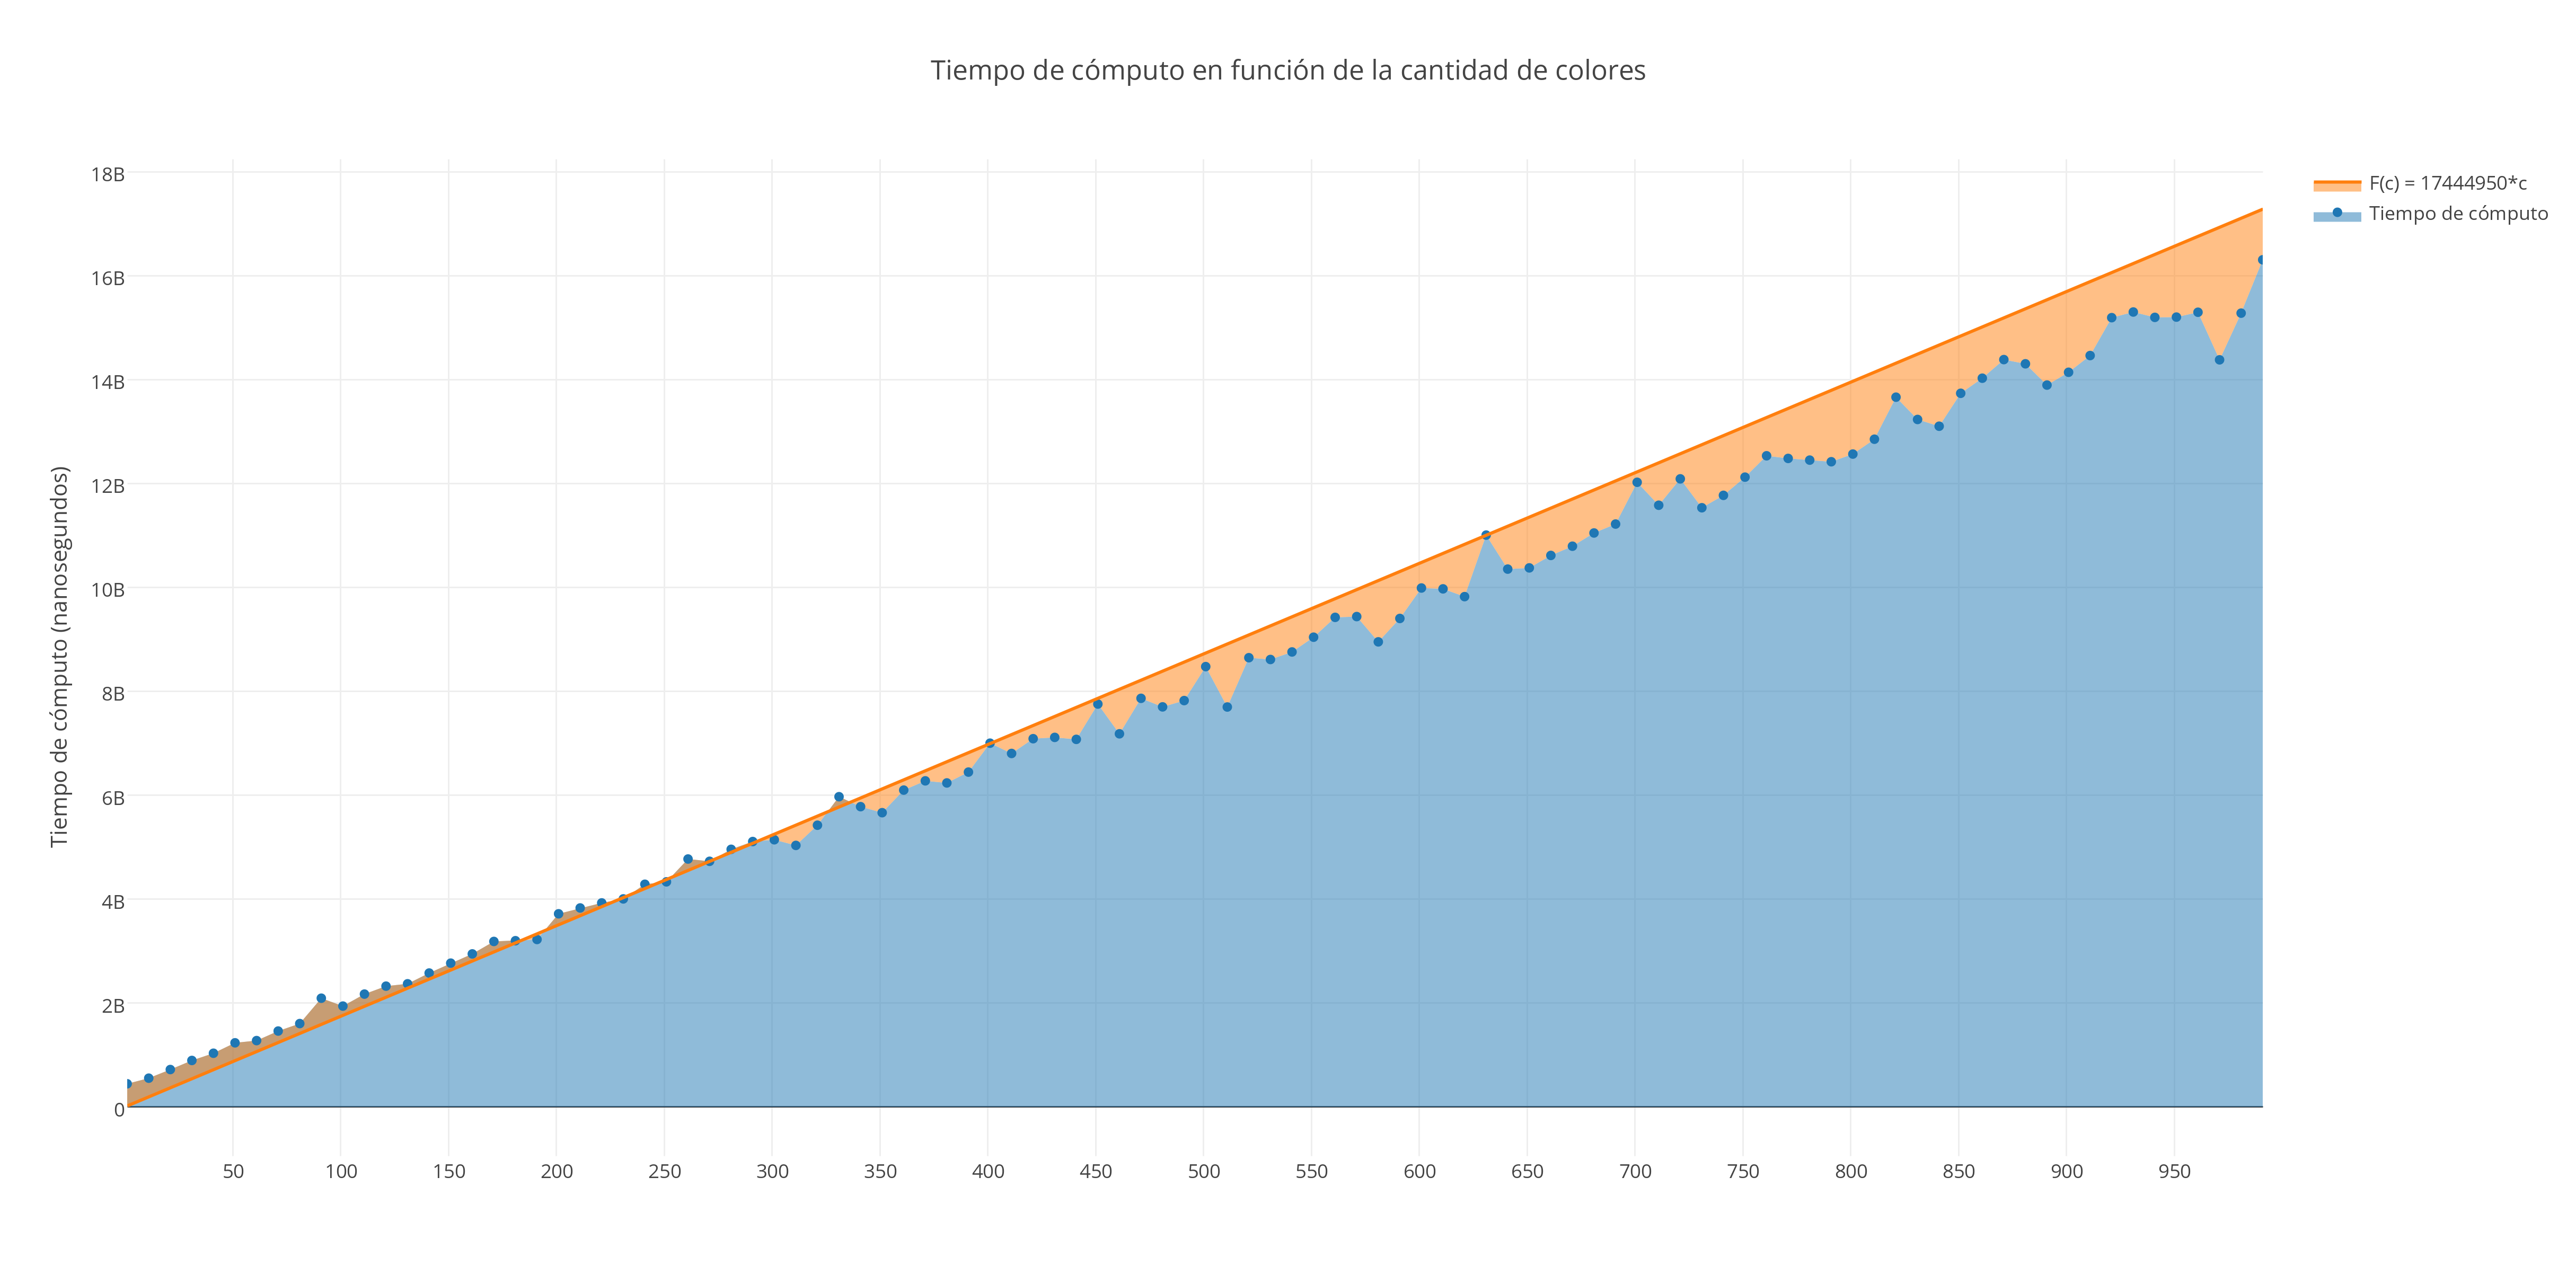
\includegraphics[width=18cm]{imagenes/Ej3/colorestiempo.png}
 	\caption{Tiempos de cómputo en función de la cantidad de colores}
 	\label{colorestiempo}
    \end{center}
  \end{figure}

La misma parece indicar que el tiempo de cómputo dependiera linealmente de la cantidad de colores máxima del grafo. Para entenderlo, hay que considerar que la elección de un color para cada vértice implica haber recorrido cada uno de sus colores. Es decir, es necesario hacer N veces C (a lo sumo). De esta forma, al incrementar la cantidad de colores se realiza una iteración más costosa por cada nodo que no deja de ser lineal.\\

Por último analizamos qué ocurre con la cantidad de conflictos presentes luego del coloreo en función de la cantidad de colores disponibles para realizarlo. Tal como esperábamos a medida que se incrementa el módulo del conjunto de colores, disminuye la cantidad de conflictos. \\
En este caso los resultados resultan intuitivos, puesto que si se dispone de un único color entonces todos aquellos nodos que tengan adyacentes generarán conflictos, puesto que todos ellos tienen una única opción para colorearse. En contrapartida, sabemos que cualquier grafo requiere para ser coloreado a lo sumo tantos colores como cantidad de vértices contenga. En un punto intermedio, como cada nodo tiene potencialmente una cantidad de restricciones intermedia, también la cantidad de conflictos se espera que sea media (es decir, si dos nodos adyacentes comparten colores, siempre existe la posibilidad de que elijan uno distinto cada uno)  \\
Los resultados se pueden observar en la imagen \ref{coloresconflicto}


 \begin{figure}[H]
    \begin{center}
  	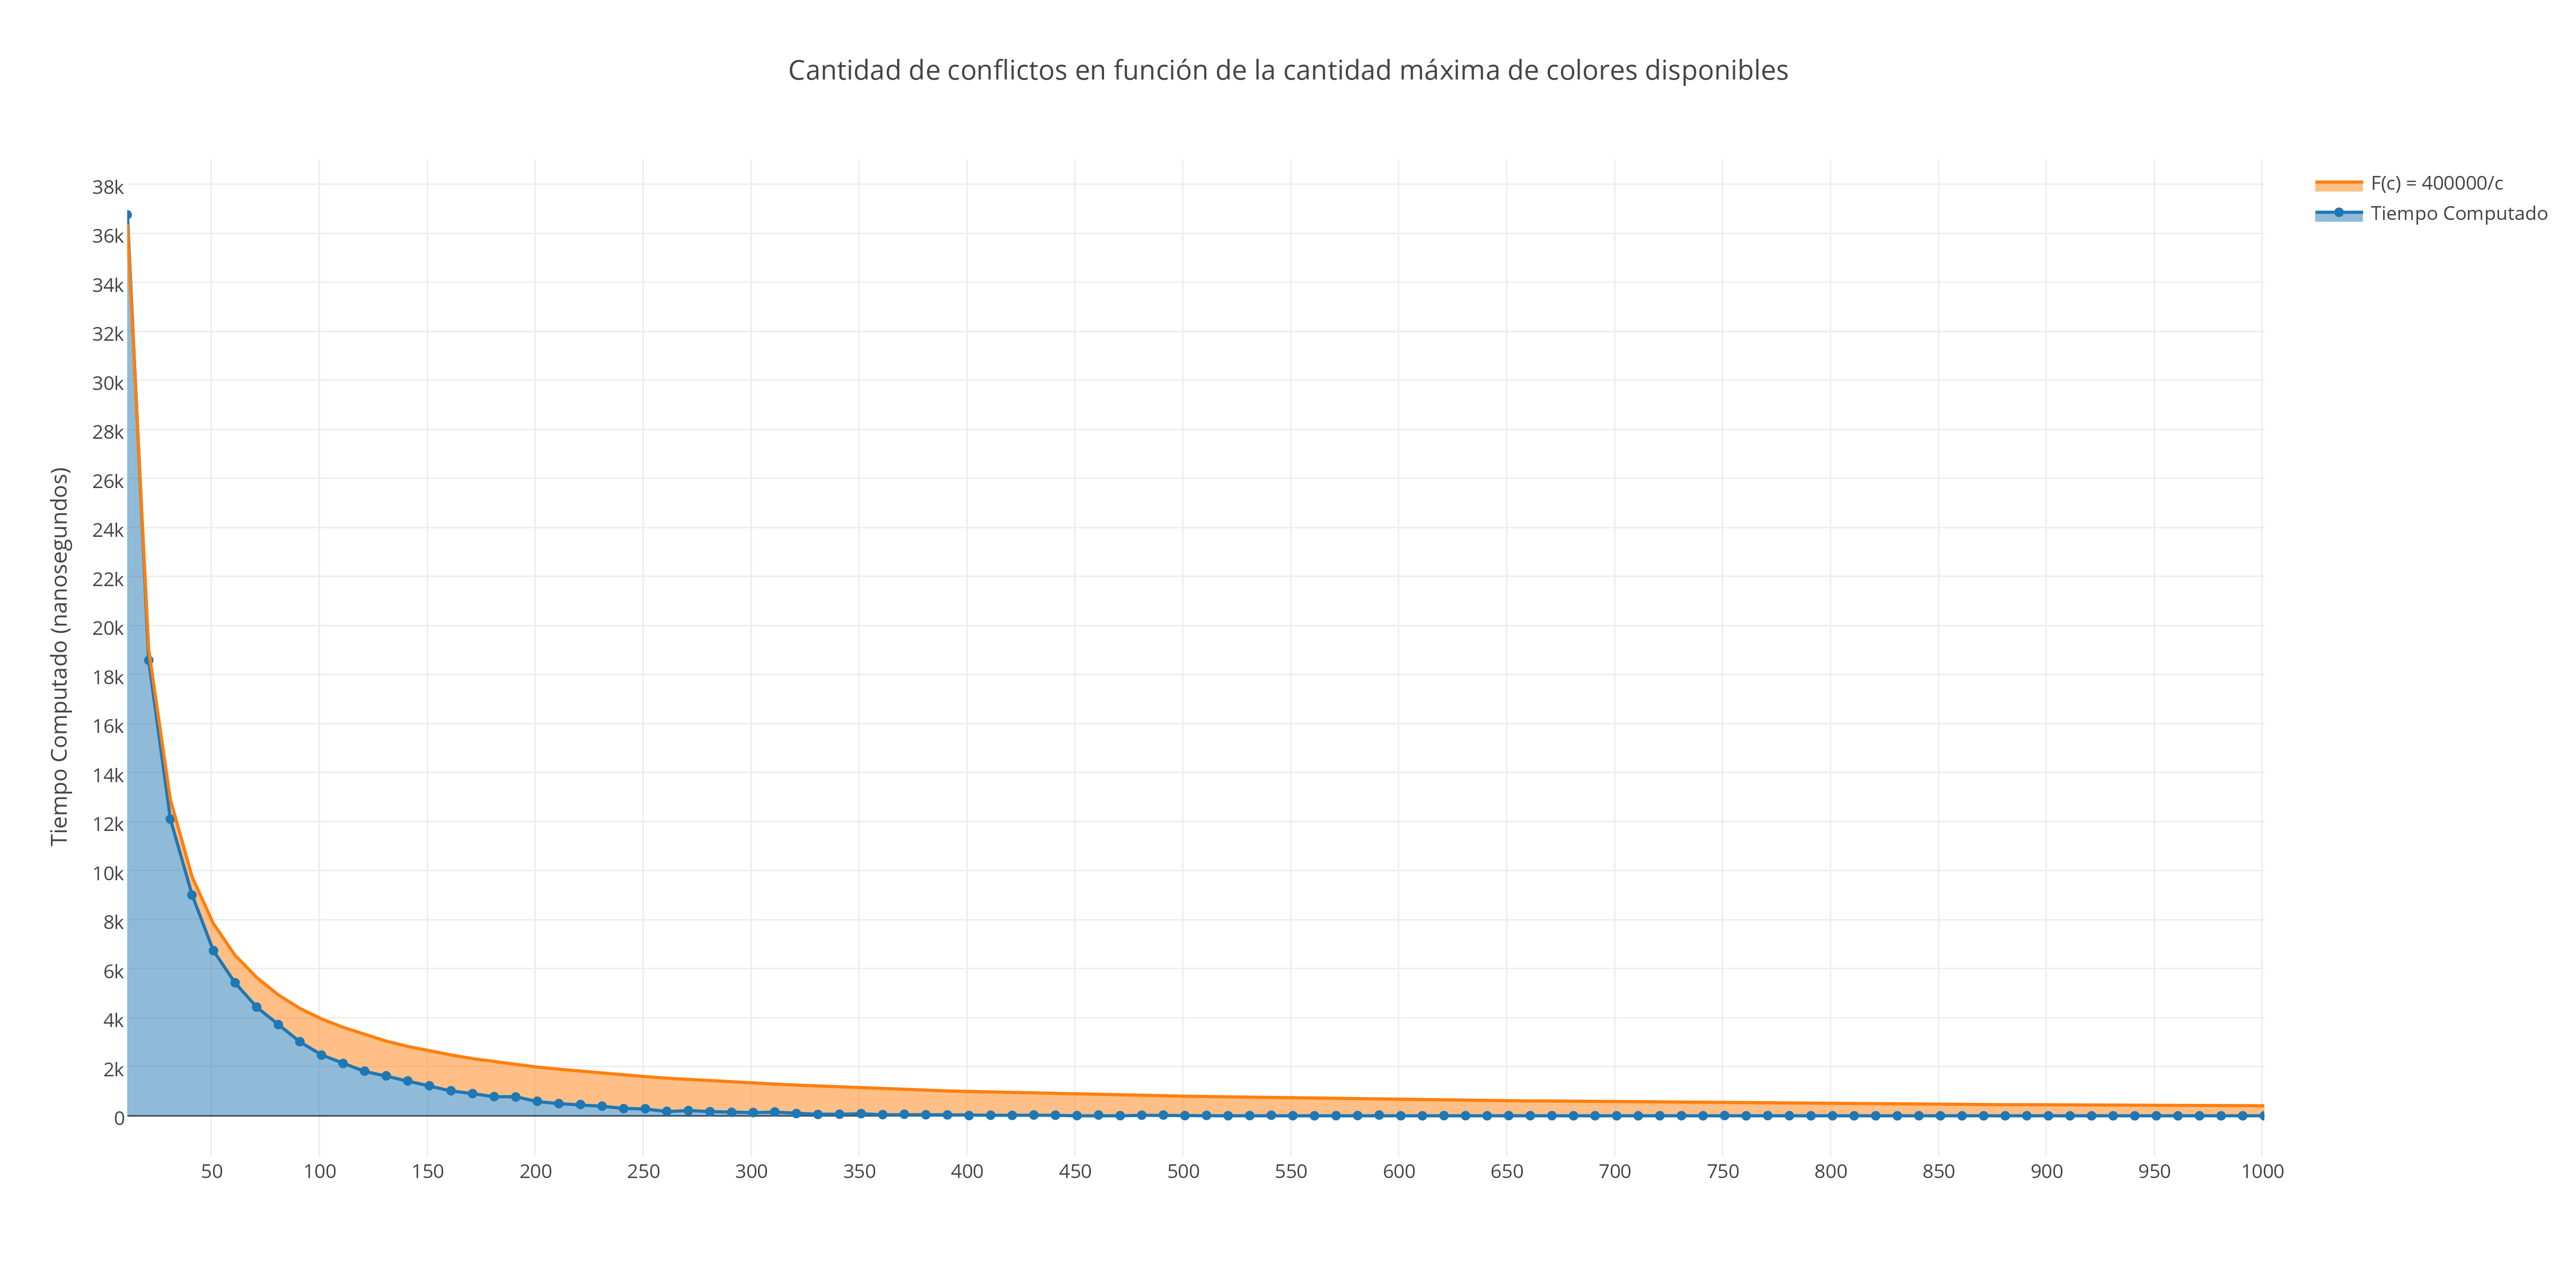
\includegraphics[width=18cm]{imagenes/Ej3/coloresconflicto.png}
 	\caption{Total de conflictos en función de la cantidad de colores máxima}
 	\label{coloresconflicto}
    \end{center}
  \end{figure}

\subsubsection{Peor caso}
Considerando la heurística propuesta, el peor caso a considerar es aquel en que todos los nodos tienen n - 1 nodos adyacentes (es decir un grafo completo). En esta situación el método PintarNodo() - que  se encarga de decidir qué color de los disponibles parecería el apropiado para cada vértice - cumple la cota teórica propuesta, pues debe hacer tantas operaciones como cantidad de vecinos del nodo que  se examina.\\

Además se debe considerar la relación entre la cantidad de colores y la de nodos, puesto que al estar la complejidad fuertemente influida por ambos valores, el que determine finalmente los tiempos de ejecución en el peor caso será aquel cuya cota inferior sea la mayor entre ambas. En otras palabras, si el valor de C fuese equivalente en cada caso a $N^{N}$  (un caso irrisorio - dado que cualquier grafo necesita a lo sumo N colores para colorearse - pero posible) entonces la cota superior estaría determinada en última instancia por el valor de C, absorbiendo asintóticamente la complejidad aportada por N. \\
Por el contrario, si C fuese menor que la cantidad de vértices entonces la cota superior de la heurística propuesta pertenecería a O( $N^{3}$ * log (N) )


\subsubsection{Mejor caso}
Por lo antedicho, el mejor caso se constituye tomando un grafo donde todos sus vértices son aislados. De esta manera, todos y cada uno de ellos podría ser coloreado indistintamente con cualquiera de sus colores disponibles. Sin embargo el conjunto de colores seguiría siendo iterado en su totalidad.



\newpage
